\documentclass[10pt]{article}
\usepackage[T1]{fontenc}
\usepackage{tgadventor}

\usepackage[margin=0.75in]{geometry}
\usepackage{multicol}
\usepackage{titlesec}
\usepackage{xcolor}
\usepackage{svg}
\usepackage{tabularx}
\usepackage{graphicx}
\usepackage{float}
\usepackage{amsmath}
\usepackage{hyperref}
\usepackage{tikz}
\usepackage{fancyhdr}
\usepackage{lastpage}
\usepackage{pgfplots}
\usepackage{subcaption}
\usepackage[american,siunitx]{circuitikz}
\usepackage[backend=biber, defernumbers=true, sorting=none]{biblatex} \nocite{*}
\usepackage[font={footnotesize,it},labelfont={footnotesize,it,bf}]{caption}
%\usepackage{indentfirst}
%\usepackage{mathptmx}

\addbibresource{references.bib}
\renewcommand*{\bibfont}{\normalfont\footnotesize}
\graphicspath{{images/}}
\setsvg{inkscapeexe={"C:/Program Files/Inkscape/bin/inkscape.exe"}} % POINT TO /inkscape.exe AS NEEDED
\newcolumntype{C}{>{\centering\arraybackslash}X} % from array package
\usetikzlibrary{positioning, shapes.geometric, patterns, patterns.meta}
\titlespacing*{\section}{0pt}{5pt}{5pt}
\titlespacing*{\subsection}{0pt}{8pt}{3pt}
\definecolor{copper}{rgb}{0.72, 0.45, 0.2}
\definecolor{forestgreen(traditional)}{rgb}{0.0, 0.27, 0.13}
\definecolor{forestgreen(web)}{rgb}{0.13, 0.55, 0.13}
\definecolor{github-indigo}{RGB}{64, 120, 192}
\definecolor{github-butterfly-bush}{RGB}{110, 84, 148}
\tikzset{
    block/.style={
        draw, minimum width = 1cm, 
        minimum height = 0.7cm, 
        align = center,
        font = \footnotesize
    }, 
    every node/.style = {node distance=0.5cm},
    line/.style = {-latex}
}

\begin{document}

    \pagestyle{fancy}
    \fancyhf{}
    \fancyhead[LH]{\footnotesize{Dynamic Range Compressor Design | Goda, Shaun}}
    \fancyhead[RH]{\footnotesize{Technical Report | \today}}
    \renewcommand{\headrulewidth}{0pt}
    \fancyfoot[C]{\footnotesize{Page \thepage\ of \pageref{LastPage}}}
    \fancypagestyle{firstpage}{
        \fancyhf{}
        \fancyfoot[C]{\footnotesize Page \thepage\ of \pageref{LastPage}}
        \renewcommand{\headrulewidth}{0pt}
    }

    \title{
        \vspace{-5ex}
        \textbf{\huge Dynamic Range Compressor Design}\\
        \textit{Technical Report in Analog Signal Processing and Discrete Circuit Design for Applications in Audible Frequency Domain}
    }

    \author{
        \textbf{\Large Shaun Goda}\\
        \textit{\normalsize Department of Electrical and Computer Engineering, Rutgers University - New Brunswick}
    }

    \date{\vspace{-5ex}} % This command effectively gets rid of the date section from \maketitle

    \maketitle

    \thispagestyle{firstpage}

    \begin{abstract}
        This technical paper examines the theory and implementation of dynamic range compressors in the realm of analog signal processing. Through tests and evaluations, we present methods for achieving efficient and high-performance compressors, where we will start with an overview of the basic building block of the compressor, its representation as a mathematical function, and various methods of implementing this through analog circuits. This paper offers an entry point for those looking to understand the fundamentals of dynamic range compression techniques while balancing the nuances of the practical methods and challenges associated with developing an electronic hardware device.
    \end{abstract}
    
    \begin{multicols*}{2}

        \textbf{
            Keywords: 
            Dynamic Range Compression, Analog Signal Processing, Circuit Design, Printed Circuit Board Design, Signal Integrity.
        }

        \section{Introduction}
            A dynamic range compressor (DRC) is an essential tool in audio processing that normalizes the loudness of a signal that has been put through. This is done by using a mechanism that attenuates signals above a set threshold, utilizing a variable gain mechanism governed by a level-detection algorithm. The process effectively lowers the volume of louder segments of the audio while maintaining the level of quieter sections, resulting in a more uniform overall loudness. This technology is widely used in various areas such as music production, live performances, and even in devices like hearing aids to improve sound quality.\par
            With the emergence of high-performance computational platforms and advancement in signal processing technologies, digital signal compression algorithms has been a de-facto standard in the industry. Digital compressors are popular in many applications, from creating music to broadcasting and beyond, as they allow for detailed manipulation of sound. The digital approach to compressors and various other signal processing tools`' has revolutionized the way we work with audio, making it easier to achieve high-quality production on your personal laptop without having access to a professional recording studios.\par
            However, despite the dominance of digital signal processing technologies, hardware compressors, where the signal is processed entirely in the analog domain, remain in use. Many audio professionals continue to prefer them for certain tasks as it has the advantage of being straightforward, avoiding some of the issues that digital formats can introduce, such as digital latency caused by AD/DA conversion or digital processing delay. Furthermore, it is advantageous in avoiding issues such as unwanted sampling artifacts and the added complexity due to its digital nature.\par
            Analog compressors are also valued for the unique qualities they can add to sound. They are known for introducing a warmth and musicality to audio that is often described as difficult to achieve with digital methods. This effect is due to the slight alterations they make to the sound, including adding minor distortions and saturation, which can make the audio feel richer and more engaging. Thus, despite the convenience and precision of digital compressors, analog compressors still hold its own place in audio production for their ability to enhance sound in a distinctive way.\par
            This paper will delve deeper into the technical nuances and design considerations that underpins an effective analog compressor. By examining the control parameters, exploring the functional building blocks, and discussing various control mechanisms, we aim to investigate the intricate balance between theory and practical application that lies in designing an analog compressor. The following sections will offer a comprehensive analysis of the compressor topology, discussing various optimization strategies in designing an ideal compressor. Through this exploration, the paper aims to highlight the critical decisions and engineering challenges involved in creating an analog compressors that not only meet the technical specifications, but also stands out as an appealing alternative to the widely used digital compressor.

        \section{Compressor Control Parameters}
            A compressor's functionality is governed by its control parameters, which allow users to configure the effect's characteristics. Key parameters include Threshold, Ratio, Attack, Release, Knee, and Side-chain, each defining a specific aspect of the compressor's behavior and its impact on the audio signal.

            % Compression ratio plot
            \noindent
            \begin{minipage}{\linewidth}
                \centering
                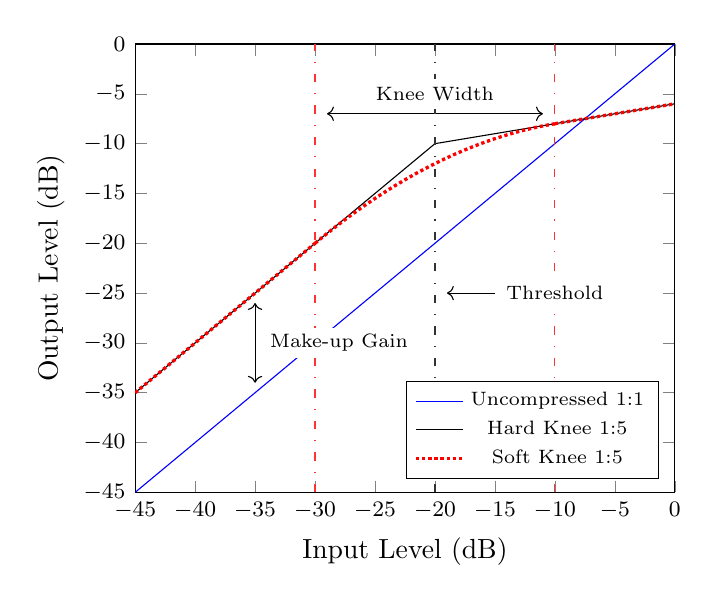
\begin{tikzpicture}
                    \begin{axis}[
                        ticklabel style = {font=\footnotesize},
                        xtick distance=5,
                        ytick distance=5,
                        xlabel={Input Level (dB)},
                        ylabel={Output Level (dB)},
                        xmin=-45, xmax=0,
                        ymin=-45, ymax=0,
                        legend pos=south east,
                        %xmajorgrids=true,
                        %ymajorgrids=true,
                        grid style=dashed,
                    ]
                    
                    % No compression line
                    \addplot[
                        color=blue,
                        domain=-45:0,
                    ] {x};
                    
                    % 5:1 Compression, hard knee
                    \addplot[
                        color=black,
                        solid,
                        domain=-45:-20,
                    ] {x + 10};
                    \addplot[
                        color=black,
                        solid,
                        domain=-20:0,
                    ] {0.2*x-6};
        
                    % 5:1 Compression, soft knee
                    \addplot[
                        color=red,
                        very thick,
                        densely dotted,
                        domain=-45:-30,
                    ] {x + 10};
                    \addplot[
                        color=red,
                        very thick,
                        densely dotted,
                        domain=-30:-10,
                    ] {-0.02*x^2-0.2*x-8};
                    \addplot[
                        color=red,
                        very thick,
                        densely dotted,
                        domain=-10:0,
                    ] {0.2*x-6};
                    
        
                    % Make-up gain
                    \draw [<->] (axis cs:-35,-34) -- (axis cs:-35,-26);

                    % Knee boundary line
                    \draw [color=red!80, loosely dashdotted] (axis cs:-30,-45) -- (axis cs:-30,0);
                    \draw [color=red!80, loosely dashdotted] (axis cs:-10,-45) -- (axis cs:-10,0);
                    \draw [<->] (axis cs:-29,-7) -- (axis cs:-11,-7);
                    
                    % Threshold line
                    \draw [color=black!80, loosely dashdotted] (axis cs:-20,-45) -- (axis cs:-20,0);
                    \draw [->] (axis cs:-15,-25) -- (axis cs:-19,-25);

                    \fill [white] (axis cs:-25,-6.5) rectangle (axis cs:-15,-3.5);
                    \node at (axis cs:-20,-5){\scriptsize{Knee Width}};

                    \fill [white] (axis cs:-15,-27) rectangle (axis cs:-5,-23);
                    \node at (axis cs:-10,-25){\scriptsize{Threshold}};

                    \fill [white] (axis cs:-34,-31.5) rectangle (axis cs:-22,-28.5);
                    \node at (axis cs:-28,-30){\scriptsize{Make-up Gain}};

                    \legend{\scriptsize{Uncompressed 1:1},,\scriptsize{Hard Knee 1:5},,\scriptsize{Soft Knee 1:5}};
                    
                    \end{axis}
                \end{tikzpicture}
                \captionof{figure}{A typical compressor's transfer characteristics.}
                \label{fig:comp-ratio}
            \end{minipage}

            \subsection{Threshold}
                The threshold parameter sets the level at which the compressor starts to act. Measured in decibels (dB), it defines the point above which the input signal will be compressed. When the signal level exceeds this threshold, compression is applied.

            \subsection{Ratio}
                The ratio determines the degree of compression applied to the signal once it surpasses the threshold. It is expressed as a ratio (e.g., 4:1, 10:1). A 4:1 ratio means that for every 4 dB, the input signal exceeds the threshold, the output signal level will be increased by only 1 dB. Higher ratios result in more aggressive compression.

            \subsection{Attack}
                The attack time is the time it takes for the compressor to start acting after the signal exceeds the threshold, as seen in the "attack phase" section of figure \ref{fig:comp-trans}. It is usually measured in milliseconds (ms). A fast attack time means the compressor responds quickly to level changes, suitable for controlling sharp, transient sounds. A slower attack allows some of the initial transients through, preserving more of the signal's natural character.

            \subsection{Release}
                Release time is the time it takes for the compressor to stop acting after the signal falls below the threshold. Also measured in milliseconds, a shorter release time stops the compression effect more quickly, which can help maintain natural dynamics but might result in a 'pumping' sound. A longer release time provides a smoother, more gradual return to the uncompressed state.
            
                % Transient response diagram
                \noindent
                \begin{minipage}{\linewidth}
                    \centering
                    \includesvg[inkscapelatex=false,width=0.935\linewidth]{attack-release-trans.svg}
                    \captionof{figure}{Transient response of a signal through a compressor.}
                    \label{fig:comp-trans}
                \end{minipage}

            \subsection{Knee}
                The knee parameter adjusts how the compressor transitions from the non-compressed to the compressed state. A 'hard knee' setting means the compression ratio is applied abruptly as soon as the signal crosses the threshold. In contrast, a 'soft knee' setting introduces compression gradually as the signal approaches and then exceeds the threshold. This results in a more natural, less noticeable compression effect.
            
            \subsection{Make-Up Gain}
                Make-up gain is a control parameter that allows you to increase the output level of the signal after it has gone through compression. This feature helps the user with adjusting the output to a consistent volume level after the signal has undergone attenuation by the compression algorithm. In the context of a song or an audio program, it allows the user to enhances the presence of the material.

            \subsection{Side-chain}
                Side-chain is a compressor control that enables external audio signals to trigger compression on another audio track. This technique allows the compressor to react not to its own input signal, but to the dynamics of another, offering creative applications such as ducking, where the volume of one sound is reduced by the presence of another (e.g., background music lowering when someone speaks). It's a powerful tool for achieving more complex mixing and mastering effects, enhancing clarity, and creating rhythmic variations in audio production.

        \section{Functional Building Blocks of a Compressor}

            \subsection{Threshold Detector}
                The threshold detector is responsible for producing the control voltage, which dictates the gain reduction level applied to the signal. This stage encompasses parameters like Threshold (T), Ratio (R), and Knee Width (W), which collectively establish the static input-output relationship for compression. When the signal level surpasses the threshold, it undergoes attenuation following the specified ratio.
            
            \subsection{Input Level Detector}
                The volume detector is responsible for providing a representation of the loudness of the input signal. There are a two main ways including the peak detector and the RMS detector to generate the control voltage based on the input.

                \subsubsection{Average Reading Level Detector}
                
                    A simple peak detection circuit can be implemented using a diode, a capacitor, and a resistor.
                    
                    % Lossy peak detector diagram
                    \noindent
                    \begin{minipage}{\linewidth}
                        \centering
                        \begin{circuitikz}[scale = 0.8, transform shape]
                            \draw
                            (0,0) node[left]{Input}
                            (0,0) to[empty diode, *-] (2,0)
                            to[R, l_=$R_A$] (4,0)
                            to[short] (5,0)
                            to[C, l_=$C$] (5,-2) node[sground]{}
                            (5,0) to[short] (6.5,0)
                            to[R, l_=$R_R$] (6.5,-2) node[sground]{}
                            (6.5,0) to[short, -*] (7.5,0)
                            (7.5,0) node[right]{Output}
                            ;
                        \end{circuitikz}
                        \captionof{figure}{Circuit diagram of a lossy peak detector.}
                        \label{fig:lossy-peak-det}
                    \end{minipage}
                    
                \subsubsection{RMS Level Detector}
                    Referencing the Root Mean Squared (RMS) value of the input signal may be useful when we would like to set the compression reference based on the smoothed average of the input signal. Unlike peak detection, 
                    
                    The RMS value in its continuous form expression is defined by the following function. \cite{aes-that-rms}
                    
                    \begin{equation}
                        V_{RMS} = \lim_{T \to \infty}\sqrt{\frac{1}{T}\int_{-\infty}^{T} v_{in}^2(t) \,\cdot dt}
                    \end{equation}
                    
                    Utilizing the RMS value of the input signal is particularly helpful when you would like to utilize a reference that is more aligned with how our ears perceive loudness. RMS detection ensures more consistent levels throughout the audio material, as it's less influenced by short transient peaks, and is suited for providing a more musical and natural-sounding compression.

                    % RMS and peak comparison table
                    \begin{table*}[!th]
                        \centering
                        \begin{tabularx}{\textwidth}{|l*{4}{|C}|}
                            \hline
                            Type of Waveform (1V Peak Amplitude) & Crest Factor $(V_{Peak}/V_{RMS})$ & RMS value & Average Reading Circuit & Error (\%) \\ \hline
                            Undistorted Sine Wave & 1.414 & 0.707 & 0.707 & 0 \\    \hline
                            Gaussian Noise & 3 & 0.333 & 0.295 & -11.4 \\   \hline
                            Undistorted Triangle Wave & 1.73 & 0.577 & 0.555 & -3.8 \\   \hline
                            Gaussian Noise (98\% of Peaks<1V) & 3 & 0.333 & 0.295 & -11.4 \\    \hline
                            Rectangular & 2 & 0.5 & 0.278 & -44 \\    \hline
                            Pulse Train & 10 & 0.1 & 0.011 & -89 \\    \hline
                            SCR Waveform (50\% Duty) & 2 & 0.354 & 0.354 & -28 \\    \hline
                            SCR Waveform (25\% Duty) & 4.7 & 0.212 & 0.150 & -30 \\    \hline
                        \end{tabularx}
                        \caption{Error introduced by an average responding circuit when measuring common waveforms.}
                        \label{table:ave-err}
                    \end{table*}
                    
                \subsubsection{Crest Factor}
                    The crest factor, representing the ratio of a signal's peak amplitude to its root mean square (RMS) value, plays a important role in the control of dynamic range compression. By quantifying the extent of peakiness in audio signals, it offers a valuable metric for adjusting the gain in dynamic range compressors, aligning more closely with the intricacies of human auditory perception. This parameter is particularly crucial in scenarios where maintaining audio fidelity is paramount, as it helps in tailoring the compression process to preserve the natural dynamics of the source material while preventing auditory fatigue in listeners.\par
                    In practical terms, the crest factor informs the design of gain control circuitry by facilitating a more discerning response to varying signal characteristics. It enables the compression algorithm to dynamically adjust its parameters, such as threshold and ratio, based on the signal's momentary peakiness rather than its average level or instantaneous peaks alone. This approach ensures a more balanced and transparent output, minimizing the risk of overcompression, which can lead to a loss of dynamic range and a 'flattened' audio experience.

                \subsubsection{Pre-Detection Filtering}
                    Broadband compressors works on the dynamics of an input signal across the entire frequency range. When a set threshold is exceeded, the entire signal is affected, regardless of which frequencies the energy of the signal is composed of.\par
                    In a multiband compressor, the entire frequency spectrum is split up into multiple bands that can be parametrized independently from each other. Hence, you are able to compress a single track or instrumental group much more flexible and heavier, without having to fear that bigger changes end up being audible too much.\par
                    With a spectral compressor, the spectral distribution of energy of a signal is analyzed continuously and compared with target values that have been calculated by intelligent algorithms. When the system recognizes that certain frequency areas are currently being overemphasized and therefore affect the compression disproportionately, these areas are automatically compressed more.

            \subsection{Gain Level Controller}
                The gain control in a dynamic range compressor can be achieved by using a voltage controlled amplifier (VCA) where its gain factor is modulated by a control voltage generated by the level detection circuitry. The VCA adjusts the signal's gain based on this control voltage, which reflects the signal's amplitude relative to the compressor's parameters (threshold, ratio, attack, release).
            
        \section{Compressor Topology}
            Compressor topology fundamentally influences the performance, sound characteristics, and functionality of dynamic range compressors. Such influences can be seen in factors such as how quickly a compressor reacts to signal changes, the smoothness or aggressiveness of compression, and how transparently it applies gain reduction. In the following section, two topology including feedback and feed-forward is discussed.

            \subsection{Feedback Compression}  
                In a feedback topology, the output signal is looped back and used as part of the signal processing chain as shown in figure ?. This configuration allows for the compressor to react to the processed signal, enabling a more adaptive response to the audio material. \textcolor{red}{Feedback topology is often praised for its musicality, as it tends to produce a more natural compression effect.} The inherent nature of the feedback system ensures that the compressor's adjustments are directly influenced by its own output, leading to a smoother and more consistent control over dynamic range. This topology excels in applications where preserving the natural dynamics and timbre of the audio is important.
                
                % Feedback diagram
                \noindent
                \begin{minipage}{\linewidth}

                    \centering

                    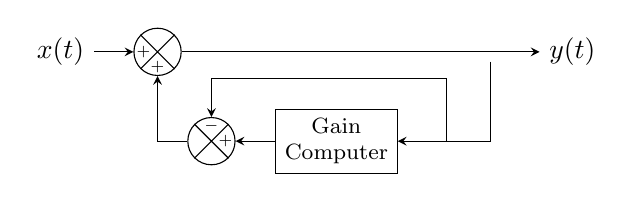
\begin{tikzpicture}

                        \node (input) at (0,0) {$x(t)$};
                        \node (output) at (6.5,0) {$y(t)$};

                        % Sum1 shape
                        \node[draw,
                            circle,
                            minimum size=0.6cm,
                            right = of input,
                        ] (sum1) {};
                        \draw (sum1.north east) -- (sum1.south west) (sum1.north west) -- (sum1.south east);
                        \node[left=-1pt] at (sum1.center){\tiny $+$};
                        \node[below] at (sum1.center){\tiny $+$};       
                        
                        % Sum2 shape
                        \node[draw,
                            circle,
                            minimum size=0.6cm,
                            below right = 0.7 and 0.25 of sum1,
                        ] (sum2) {};
                        \draw (sum2.north east) -- (sum2.south west) (sum2.north west) -- (sum2.south east);
                        \node[above] at (sum2.center){\tiny $-$};
                        \node[right=-1pt] at (sum2.center){\tiny $+$};
            
                        % Gain Computer
                        \node[block, right = of sum2] (gain) {Gain\\Computer};

                        % Lines
                        \draw[-stealth] (input) -- (sum1.west);
                        \draw[-stealth] (sum1.east) -- (output) node[left = of output](split1){};
                        \draw[-stealth] (sum2.west) -| (sum1.south);
                        \draw[-stealth] (gain.west) -- (sum2.east);
                        \draw[-stealth] (split1) |- (gain.east) node[right = of gain](split2){};
                        \draw[-stealth] (split2) -| +(0,0.8) -| (sum2.north);
                        
                    \end{tikzpicture}
                        
                    \captionof{figure}{Control diagram of a feedback compressor topology.}
                    \label{fig:feedback}
                
                \end{minipage}
                
            \subsection{Feed-forward Compression}
                As opposed to the feedback topology, feed-forward topology uses the input signal directly to control the compression process, without the influence of the compressed signal in the control loop. \ref{fig:feedforward} This allows for more precise and immediate control over the compression characteristics, as the system's response is solely based on the incoming audio signal. \textcolor{red}{Feed-forward compressors are known for their accuracy and fast response, making them ideal for applications requiring precise dynamic control, such as in limiting scenarios where preventing signal peaks is crucial.}\par

                % Feed-forward diagram
                \noindent
                \begin{minipage}{\linewidth}

                    \centering

                    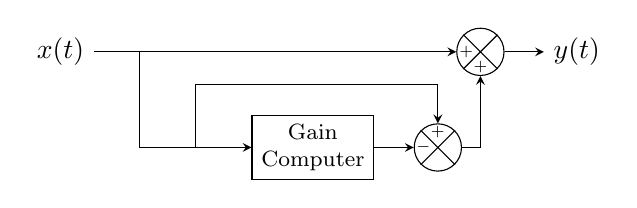
\begin{tikzpicture}

                        \node (input) at (0,0) {$x(t)$};

                        % Gain Computer
                        \node[block, below right = 0.5 and 2 of input] (gain) {Gain\\Computer};

                        % Sum1 shape
                        \node[draw,
                            circle,
                            minimum size =0.6cm,
                            right = of gain,
                        ] (sum1) {};
                        \draw (sum1.north east) -- (sum1.south west) (sum1.north west) -- (sum1.south east);
                        \node[left=-1pt] at (sum1.center){\tiny $-$};
                        \node[above] at (sum1.center){\tiny $+$};       
                        
                        % Sum2 shape
                        \node[draw,
                            circle,
                            minimum size = 0.6cm,
                            right = 4.6cm of input,
                        ] (sum2) {};
                        \draw (sum2.north east) -- (sum2.south west) (sum2.north west) -- (sum2.south east);
                        \node[left=-1pt] at (sum2.center){\tiny $+$};
                        \node[below] at (sum2.center){\tiny $+$};
            
                        % Lines
                        \draw[-stealth] (input) -- (sum2.west);
                        \draw[-stealth] (1,0) |- (gain.west) node[near end](split){};
                        \draw[-stealth] (gain.east) -- (sum1.west);
                        \draw[-stealth] (split) -| +(0,0.8) -| (sum1.north);
                        \draw[-stealth] (sum1.east) -| (sum2.south);
                        \draw[-stealth] (sum2.east) -- +(0.5,0) node[right]{$y(t)$};
                        
                    \end{tikzpicture}
                    
                    \captionof{figure}{Control diagram of a feed-forward compressor topology.}
                    \label{fig:feedforward}
                
                \end{minipage}
        
        \section{Optimization of the Compressor Architecture}
            
            \subsection{Logarithmic Domain Signal Processing}
                \textcolor{blue}{A log domain amplifier can be implemented so that we can operate mathematical operations such as multiplication and division on analog signals. This can be done as summation and subtraction in the log domain directly translate to multiplication and division once converted back to its linear representation.}

                The discharge of a capacitor is expressed by the following equation.              
                
                \begin{equation}
                    V(t) = V_0 e^{-\frac{t}{RC}}
                \end{equation}    
                
                This equation shows that the decay in the voltage of a capacitor is represented as an exponential function.
                When we take the natural logarithm of the function on both sides, we will get the expression shown below.
                
                \begin{equation}
                    \ln(V(t)) = \ln(V_0) - \frac{t}{RC}
                \end{equation}
                
                Since we are relying on discrete circuitry to implement the compressor, we would have to take the discharge characteristic of capacitive elements into our calculation.

            \subsection{Mixed Use of Averaging and RMS Level as an Input Level Reference}

            \subsection{Compressor Topology Selection}

                % Control diagram of compressor to be implemented
                \begin{figure*}[!th]

                    \centering
                    
                    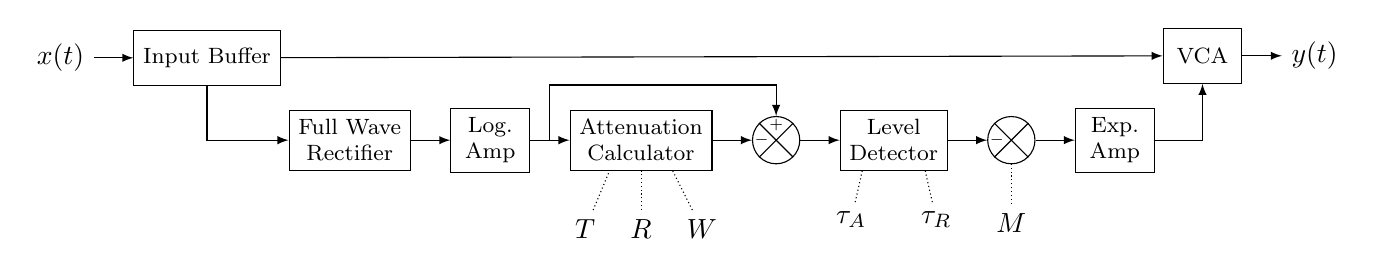
\begin{tikzpicture}
                            
                        \node (input) at (0,0) {$x(t)$};
                                                
                        % Blocks
                        \node[block, right = of input] (inBuf) {Input Buffer};
                        \node[block, below right = 0.3 and 0.1 of inBuf] (abs) {Full Wave \\ Rectifier};
                        \node[block, right = of abs] (log) {Log. \\ Amp};
                        \node[block, right = of log] (th) {Attenuation \\ Calculator};

                        % Sum1 shape
                        \node[draw,
                            circle,
                            minimum size=0.6cm,
                            right = of th,
                        ] (sum1) {};
                        \draw (sum1.north east) -- (sum1.south west) (sum1.north west) -- (sum1.south east);
                        \node[left=-1pt] at (sum1.center){\tiny $-$};
                        \node[above] at (sum1.center){\tiny $+$}; 

                        %\node[block, below = of peak] (rms) {RMS Detector};
                        \node[block, right = of sum1] (peak) {Level \\ Detector};
                        
                        % Sum2 shape
                        \node[draw,
                            circle,
                            minimum size=0.6cm,
                            right = of peak,
                        ] (sum2) {};
                        \draw (sum2.north east) -- (sum2.south west) (sum2.north west) -- (sum2.south east);
                        \node[left=-1pt] at (sum2.center){\tiny $-$};

                        % Additional blocks
                        \node[block, right = of sum2] (antilog) {Exp. \\ Amp};
                        \node[block, above right = 0.3 and 0.1 of antilog] (vca) {VCA};
                        \node[right = of vca] (output) {$y(t)$};

                        % Lines
                        \draw[line] (input.east) -- (inBuf);
                        \draw[line] (inBuf) |- (abs);
                        \draw[line] (abs) -- (log);
                        \draw[line] (log) -- (th) node[midway](split) {};
                        \draw[line] (th) -- (sum1.west);
                        \draw[line] (split) -| +(0,0.7) -| (sum1.north);
                        \draw[line] (sum1.east) -- (peak);
                        \draw[line] (peak) -- (sum2.west);
                        \draw[line] (sum2.east) -- (antilog);
                        \draw[line] (antilog) -| (vca);
                        \draw[line] (inBuf) -- (vca);
                        \draw[line] (vca) -- (output);        

                        % Arrows and labels for T, R, W
                        \node[below = 0.5cm of th] (r) {$R$};
                        \node[left = 0.2cm of r] (t) {$T$};
                        \node[right = 0.2cm of r] (w) {$W$};
                        \draw[densely dotted] (t) -- ([xshift=-0.4cm]th.south);
                        \draw[densely dotted] (r) -- (th.south);
                        \draw[densely dotted] (w) -- ([xshift=0.4cm]th.south);

                        % Arrows and labels for tau_A, tau_R
                        \node[below = 0.5cm of peak] (cent) {};
                        \node[left = 0.1cm of cent] (tauA) {$\tau_A$};
                        \node[right = 0.1cm of cent] (tauR) {$\tau_R$};
                        \draw[densely dotted] (tauA) -- ([xshift=-0.4cm]peak.south);
                        \draw[densely dotted] (tauR) -- ([xshift=0.4cm]peak.south);
                        
                        % Arrows and labels for M
                        \node[below = 0.5cm of sum2] (m) {$M$};
                        \draw[densely dotted] (m) -- (sum2.south);
                        
                    \end{tikzpicture}

                    \caption{Control diagram of proposed DRC system.}
                    \label{fig:drc-diagram}

                \end{figure*}

                Both feedback and feedforward topologies offer unique benefits and are chosen based on the specific requirements of the application. The selection between feedback and feedforward topology affects aspects such as the compressor's responsiveness, the ease of implementation, and the overall sound character. Integrating these topologies within the broader system design, taking into account control systems theory and practical implementation considerations, is essential for optimizing the compressor's performance and achieving the desired dynamic range control.\par
                \textcolor{blue}{According to a paper by Giannoulis et al. \cite{drc-tutorial}, "the detector directly smooths the control voltage instead of the input signal." Since the control voltage automatically returns back to zero when the compressor does not attenuate, we do not depend on a fixed threshold, and a smooth release envelope is guaranteed. The trajectory now behaves exponentially in the decibel domain, which means that the release time is independent of the actual amount of compression. This behavior seems smoother to the ear since the human sense of hearing is roughly logarithmic.} 

                \begin{eqnarray}
                    x_G(t)&=&20log_{10}|x(t)|\\
                    x_L(t)&=&x_G(t)-y_G(t)\\
                    x_{dB}(t)&=&-y_L(t)
                \end{eqnarray}
                        
        \section{Circuit Implementation}

            \subsection{Precision Full-Wave Rectifier}
                A precision full-wave rectifier has been implemented to feed the absolute value of the input signal into the level detection circuitry. This is necessary as the level detection circuitry could detect signals only over positive ranges. By converting a signal that ranges over the negative and positive ranges into a signal that is represented only in the positive domain, the level detector can output a value that represents the energy of the entire signal instead of half of it.
                
            \subsection{Logarithmic and Exponential Amplifiers}
                \textcolor{blue}{Explain the difference in exponential decay vs linear decay and its significance. I plan to implement the circuit that appears in an application report \cite{ti-log-conv} by Texas Instruments.}
                \textcolor{blue}{This circuit reverts the signal that has converted to dB scale back into the linear domain signal.}
            
            \subsection{Input Level Detector}

                \subsubsection{Precision Peak Detector}
                    \textcolor{blue}{This is an alternative to the RMS detector. However, it excels at fast attack signals compared to the RMS detector. This allows the compressor to process signals at higher speeds instead of simply normalizing the volume.}  

                \subsubsection{True RMS Detector}
                    A traditional approach to reading the average of an input signal was to implement a 
                    
                    For the RMS detector, an LTC1966 true-RMS detector by Analog Devices will be used. The LTC1966 utilizes a $\Delta\Sigma$ computational technology patented by Analog Devices, which makes it simpler to use, more accurate, requires less power, and is dramatically more flexible than the conventional log anti-log RMS-to-DC converters.                          
            
                \subsubsection{Detection Level Mixing}
                    Introducing a mixer that allows smooth adjustment between RMS level and peak detected level offers enhanced flexibility for dynamic control, enabling more tailored responses to different audio materials. This feature allows for better transient shaping, smoother gain reduction, and more consistent handling of varied material, from preserving the punch of percussive elements to ensuring vocal and instrumental lines are evenly balanced. Notable analog compressors like the Empirical Labs Distressor and the Manley Variable Mu leverage such capabilities, providing users with a powerful tool for both technical precision and creative expression in audio processing. This blending feature significantly expands the creative possibilities, making these compressors highly valued for their ability to adapt to and enhance a wide range of audio material.

                \subsubsection{Pre-Detection Filtering}
                    Pre-detection filtering can be introduced to limit the range of frequency the compressor is responsible for running the detection. This is particularly useful in emphasizing or de-emphasizing certain frequencies, thereby making the compressor more sensitive or less sensitive to those frequencies. As an example, a high-pass filter might be applied to prevent low-frequency content from triggering the compression, which is particularly useful for avoiding unnecessary compression due to bass-heavy elements in a mix. Pre-detection filtering allows for more targeted and musically relevant compression by controlling which parts of the frequency spectrum most influence the compressor's action, leading to a more controlled dynamic response.


            \subsection{Knee Level Management}
                The continuous output function of a compressor with knee control can be described by the following set of continuous functions.

                % Expression of knee control in terms of 
                \begin{equation}
                    y=
                    \begin{cases}
                        \frac{x-T}{R}+T & \text{for $2(x-T)>W$}\\[5pt]
                        \frac{(x-T+\frac{W}{2})^2(\frac{1}{R}-1)}{2W}+x & \text{for $2\left\lvert x-T\right\rvert\leq W$}\\[5pt]
                        x & \text{for $2(x-T)<-W$}
                    \end{cases}
                \end{equation}

                \subsubsection{Precision Clipper}

                    % Feed-forward diagram
                    \noindent
                    \begin{minipage}{\linewidth}

                        \centering

                        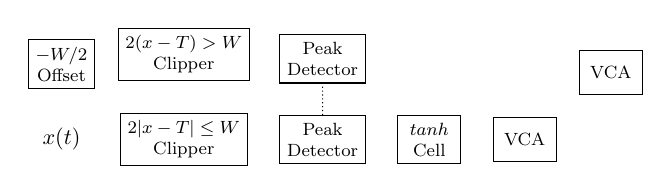
\begin{tikzpicture}[scale = 0.8, transform shape]

                            \node (input) at (0,0) {$x(t)$};
                            \node[block, right = of input] (clip+-) {$2|x-T|\leq W$\\Clipper};
                            \node[block, above = of input] (offset) {$-W/2$\\Offset};
                            \node[block, above = of clip+-] (clip-) {$2(x-T)>W$\\Clipper};
                            \node[block, right = of clip+-] (peak1) {Peak\\Detector};
                            \node[block, above = of peak1] (peak2) {Peak\\Detector};
                            \node[block, right = of peak1] (tanh) {$tanh$ \\Cell};
                            \node[block, right = of tanh] (vca1) {VCA};
                            \node[block, above right = of vca1] (vca2) {VCA};
                            

                            \draw[densely dotted] (peak1.north) -- (peak2.south);
                            
                        \end{tikzpicture}

                        \captionof{figure}{Knee control scheme}
                        \label{fig:knee-control}

                    \end{minipage}

                \subsubsection{Hyperbolic Tangent Function Cell}
                    A hyperbolic tangent function can be achieved in the analog signal domain by implementing a differential transistor pair coupled with an input of an operational amplifier.
                    As the input range of the function cell is determined by the voltage range of the active region given by the base input of the bipolar junction transistor, it is crucial to normalize the amplitude of the signal entering the cell beforehand. As seen in figure \ref{plot:tanh}, the gated nature of BJT input allows us to create unique characteristics in the definition of how the knee control is applied.

                    % tanh plot
                    \noindent
                    \begin{minipage}{\linewidth}

                        \centering
                        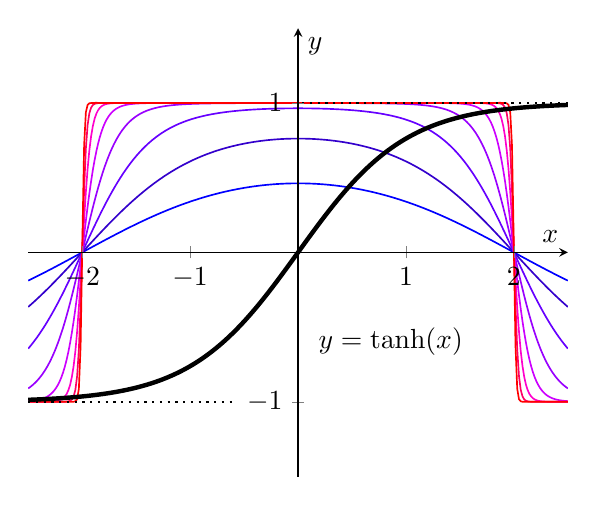
\begin{tikzpicture}
                            \begin{axis}[
                                    xmin=-2.5, xmax=2.5,
                                    ymin=-1.5, ymax=1.5,
                                    axis lines=center,
                                    axis on top=true,
                                    domain=-2.5:2.5,
                                    samples=310,
                                    ylabel=$y$,
                                    xlabel=$x$,
                                ]
                                \definecolor{c1}{HTML}{0000FF}
                                \definecolor{c2}{HTML}{3300CC}
                                \definecolor{c3}{HTML}{6600FF}
                                \definecolor{c4}{HTML}{9900FF}
                                \definecolor{c5}{HTML}{CC00FF}
                                \definecolor{c6}{HTML}{FF00CC}
                                \definecolor{c7}{HTML}{FF0066}
                                \definecolor{c8}{HTML}{FF0000}

                                \addplot [mark=none,draw=c1,semithick] {tanh(0.5*cos(deg(x)*1/4*pi))};
                                \addplot [mark=none,draw=c2,semithick] {tanh(cos(deg(x)*1/4*pi))};
                                \addplot [mark=none,draw=c3,semithick] {tanh(2*cos(deg(x)*1/4*pi))};
                                \addplot [mark=none,draw=c4,semithick] {tanh(4*cos(deg(x)*1/4*pi))};
                                \addplot [mark=none,draw=c5,semithick] {tanh(8*cos(deg(x)*1/4*pi))};
                                \addplot [mark=none,draw=c6,semithick] {tanh(16*cos(deg(x)*1/4*pi))};
                                \addplot [mark=none,draw=c7,semithick] {tanh(32*cos(deg(x)*1/4*pi))};
                                \addplot [mark=none,draw=c8,semithick] {tanh(64*cos(deg(x)*1/4*pi))};
                            
                                \addplot [mark=none,draw=black,ultra thick] {tanh(\x)};
                                \node [right, black] at (axis cs:0.1,-0.6) {$y = \tanh (x)$};
                                
                                %% Add the asymptotes
                                \draw [black, dotted, thick] (axis cs:-2.5,-1) -- (axis cs:-0.6,-1);
                                \draw [black, dotted, thick] (axis cs:+2.5,+1) -- (axis cs:0,+1);
                            \end{axis}
                        \end{tikzpicture}
                            
                        \captionof{figure}{The black line shows the function plot of $y=tanh(x)$. The red line on the other hand represents the transient output of the tanh function where amplitude of the sinusoidal input is varied.}
                        \label{plot:tanh}
                    
                    \end{minipage}

                \subsubsection{Precision Current Sink Source}
                    A current source is required to generate a constant ink of current across the collector and the emitter of the BJT being used in the tanh function cell.
                    We utilize the design shown in \cite{ti-sink-source}.

            \subsection{Voltage Controlled Amplifier}

        \section{Hardware Design}
            \textcolor{blue}{I plan to use Altium Designer for designing the PCB. Describe steps taken during the PCB design process and any important points noticed.}

            \subsection{Miscellaneous Circuitry}

                \subsubsection{Power Delivery}
                    Audio domain applications gain advantages from utilizing a bipolar bias power supply. Such a supply enhances the effective utilization of IC's full dynamic range, facilitates rail-to-rail amplification, shields the analog signal from ground noise, and delivers numerous additional benefits. \cite{ti-3-v-rails}\par
                    To receive the benefits of a split rail power supply while reducing unwanted noise and ripples seen in common topologies such as a simple switching mode power supply, a topology where a inverting charge pump is combined with an linear \& low-dropout (LDO) regulator. (shown in figure)\par
                    \textcolor{blue}{Discuss the difference in LDO over traditional power regulation sources. The DRC circuit will require a DC power source that will be converted to several voltage domains (+12V, -12V, 5V).}
                    
                    % Power management scheme diagram
                    \noindent
                    \begin{minipage}{\linewidth}

                        \centering

                        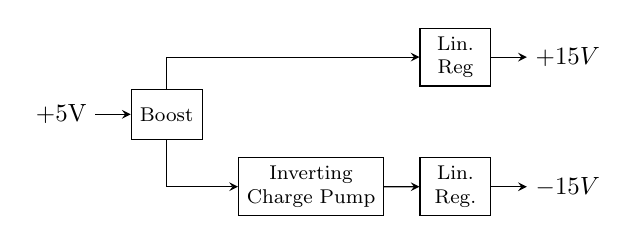
\begin{tikzpicture}[scale = 0.9, transform shape]

                            \node (input) at (0,0) {+5V};
                            \node[block, right = of input] (boost) {Boost};
                            \node[block, below right = 0.25 and 0.5 of boost] (icp) {Inverting\\Charge Pump};
                            \node[block, right = of icp] (n-ldo) {Lin.\\Reg.};
                            \node[block, above = 1 of n-ldo] (p-ldo) {Lin.\\Reg};

                            \draw[-stealth] (input) -- (boost.west);
                            \draw[-stealth] (boost.south) |- (icp.west);
                            \draw[-stealth] (boost.north) |- (p-ldo.west);
                            \draw[-stealth] (icp.east) -- (n-ldo.west);
                            \draw[-stealth] (p-ldo.east) -- +(0.5,0) node[right]{$+15V$};
                            \draw[-stealth] (n-ldo.east) -- +(0.5,0) node[right]{$-15V$};

                            %\node[block, above = of p-ldo] (p-ldo2) {Lin.\\Reg.};
                            %\draw[-stealth] (boost.north) |- (p-ldo2.west);
                            %\draw[-stealth] (p-ldo2.east) -- +(0.5,0) node[right]{$+5V$};

                        \end{tikzpicture}

                        \captionof{figure}{Power Managemenet Schema}
                        \label{fig:pwr-mng}

                    \end{minipage}

                \subsubsection{Balance Line Input/Output}

            \subsection{Printed Circuit Board Design}

                \subsubsection{Layer Stackup}
                    With the emergence of low-cost off-shore PCB manufacturing services, PCBs are easily in the reach of an average consumer who are looking to design and produce a small quantity of electronic hardware. Due to the low-cost of 2 layer and 4 layer PCBs, a 4 layer PCB can be selected as its flexible in the routing of traces and offer better signal integrity.\par
                    The three PCB stackups depicted in figure \ref{fig:pcb-stackup}, each offers distinct advantages for power delivery and signal integrity across dual power domains. The outer GND stackup provides superior EMI shielding by enclosing signal and power layers within ground planes, ensuring stable signal propagation but potentially increasing PDN inductance due to distant power planes. The one-sided hybrid stackup allows for a compact design, situating power close to its loads on one side but risking signal integrity due to the lack of adjacent ground planes. Finally, the inner GND stackup optimizes for both power integrity, with closely coupled power and ground planes minimizing PDN impedance, and signal integrity, as signals are tightly sandwiched between grounds, albeit at the potential cost of less effective EMI shielding compared to the outer GND configuration. Each stackup requires a tailored approach to manage the complexities of positive and negative power rails, thermal performance, and mechanical robustness.

                    % PCB stackup layer comparison
                    \begin{figure*}[ht]

                        \centering

                        \begin{subfigure}[b]{0.3333\linewidth}
                            \centering
                            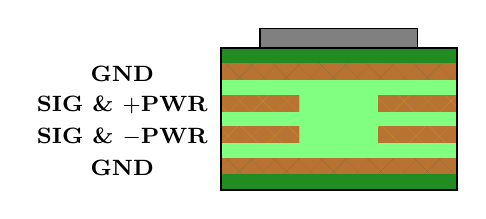
\begin{tikzpicture}
                                
                                % Light green background
                                \fill[green!50] (0,-1.4) rectangle ++(3,1);

                                % Top soldermask
                                \fill[forestgreen(web)] (0,-0.2) rectangle ++(3,0.2);

                                % S1
                                \path[fill = copper,
                                    postaction={pattern={Lines[angle=45,line width=12pt,distance={6pt}]},pattern color=forestgreen(traditional)},
                                    postaction={pattern={Lines[angle=45,line width=12pt,distance={6pt},xshift=6pt]},pattern color=copper}
                                ] (0,-0.4) rectangle ++(3,0.2);

                                % S3
                                \path[fill = red,
                                    postaction={pattern={Lines[angle=45,line width=12pt,distance={6pt}]},pattern color=yellow},
                                    postaction={pattern={Lines[angle=45,line width=12pt,distance={6pt},xshift=6pt]},pattern color=copper}
                                ] (0,-0.8) rectangle ++(1,0.2);
                                \path[fill = red,
                                    postaction={pattern={Lines[angle=45,line width=12pt,distance={6pt}]},pattern color=yellow},
                                    postaction={pattern={Lines[angle=45,line width=12pt,distance={6pt},xshift=6pt]},pattern color=copper}
                                ] (2,-0.8) rectangle ++(1,0.2);
                                
                                % S5
                                \path[fill = blue,
                                    postaction={pattern={Lines[angle=45,line width=12pt,distance={6pt}]},pattern color=yellow},
                                    postaction={pattern={Lines[angle=45,line width=12pt,distance={6pt},xshift=6pt]},pattern color=copper}
                                ] (0,-1.2) rectangle ++(1,0.2);
                                \path[fill = blue,
                                    postaction={pattern={Lines[angle=45,line width=12pt,distance={6pt}]},pattern color=yellow},
                                    postaction={pattern={Lines[angle=45,line width=12pt,distance={6pt},xshift=6pt]},pattern color=copper}
                                ] (2,-1.2) rectangle ++(1,0.2);
                                
                                % S7
                                \path[fill = copper,
                                    postaction={pattern={Lines[angle=45,line width=12pt,distance={6pt}]},pattern color=forestgreen(traditional)},
                                    postaction={pattern={Lines[angle=45,line width=12pt,distance={6pt},xshift=6pt]},pattern color=copper}
                                ] (0,-1.6) rectangle ++(3,0.2);

                                % Bottom soldermask
                                \fill[forestgreen(web)] (0,-1.8) rectangle ++(3,0.2);

                                % Outline
                                \path[draw, semithick] (0,-1.8) rectangle ++(3,1.8);

                                % Component
                                \fill[gray!100] (0.5,0) rectangle ++(2,0.25);
                                \path[draw, semithick] (0.5,0) rectangle ++(2,0.25);

                                % Labels
                                \node at (-1.25,-0.325) {\footnotesize\bf GND};
                                \node at (-1.25,-0.725) {\footnotesize\bf SIG \& $+$PWR};
                                \node at (-1.25,-1.125) {\footnotesize\bf SIG \& $-$PWR};
                                \node at (-1.25,-1.525) {\footnotesize\bf GND};

                            \end{tikzpicture}
                            \caption{{Outer GND stackup.}}
                        \end{subfigure}\hfill
                        \begin{subfigure}[b]{0.3333\linewidth}
                            \centering
                            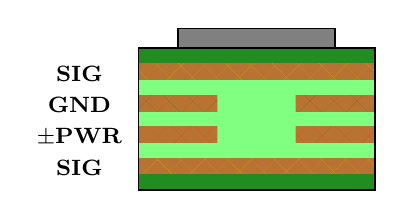
\begin{tikzpicture}
                                
                                % Light green background
                                \fill[green!50] (0,-1.4) rectangle ++(3,1);

                                % Top soldermask
                                \fill[forestgreen(web)] (0,-0.2) rectangle ++(3,0.2);

                                % S1
                                \path[fill = copper,
                                    postaction={pattern={Lines[angle=45,line width=12pt,distance={6pt}]},pattern color=yellow},
                                    postaction={pattern={Lines[angle=45,line width=12pt,distance={6pt},xshift=6pt]},pattern color=copper}
                                ] (0,-0.4) rectangle ++(3,0.2);

                                % S3
                                \path[fill = copper,
                                    postaction={pattern={Lines[angle=45,line width=12pt,distance={6pt}]},pattern color=forestgreen(traditional)},
                                    postaction={pattern={Lines[angle=45,line width=12pt,distance={6pt},xshift=6pt]},pattern color=copper}
                                ] (0,-0.8) rectangle ++(1,0.2);
                                \path[fill = copper,
                                    postaction={pattern={Lines[angle=45,line width=12pt,distance={6pt}]},pattern color=forestgreen(traditional)},
                                    postaction={pattern={Lines[angle=45,line width=12pt,distance={6pt},xshift=6pt]},pattern color=copper}
                                ] (2,-0.8) rectangle ++(1,0.2);
                                
                                % S5
                                \path[fill = blue,
                                    postaction={pattern={Lines[angle=45,line width=12pt,distance={6pt}]},pattern color=red},
                                    postaction={pattern={Lines[angle=45,line width=12pt,distance={6pt},xshift=6pt]},pattern color=copper}
                                ] (0,-1.2) rectangle ++(1,0.2);
                                \path[fill = blue,
                                    postaction={pattern={Lines[angle=45,line width=12pt,distance={6pt}]},pattern color=red},
                                    postaction={pattern={Lines[angle=45,line width=12pt,distance={6pt},xshift=6pt]},pattern color=copper}
                                ] (2,-1.2) rectangle ++(1,0.2);
                                
                                % S7
                                \path[fill = copper,
                                    postaction={pattern={Lines[angle=45,line width=12pt,distance={6pt}]},pattern color=yellow},
                                    postaction={pattern={Lines[angle=45,line width=12pt,distance={6pt},xshift=6pt]},pattern color=copper}
                                ] (0,-1.6) rectangle ++(3,0.2);

                                % Bottom soldermask
                                \fill[forestgreen(web)] (0,-1.8) rectangle ++(3,0.2);

                                % Outline
                                \path[draw, semithick] (0,-1.8) rectangle ++(3,1.8);

                                % Component
                                \fill[gray!100] (0.5,0) rectangle ++(2,0.25);
                                \path[draw, semithick] (0.5,0) rectangle ++(2,0.25);

                                % Labels
                                \node at (-0.75,-0.325) {\footnotesize\bf SIG};
                                \node at (-0.75,-0.725) {\footnotesize\bf GND};
                                \node at (-0.75,-1.125) {\footnotesize\bf $\pm$PWR};
                                \node at (-0.75,-1.525) {\footnotesize\bf SIG};

                            \end{tikzpicture}
                            \caption{{One-sided hybrid stackup.}}
                        \end{subfigure}\hfill
                        \begin{subfigure}[b]{0.3333\linewidth}
                            \centering
                            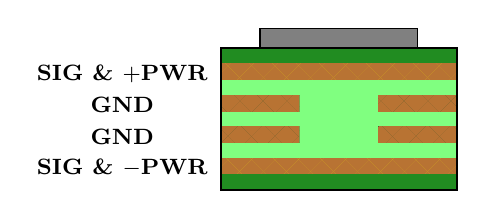
\begin{tikzpicture}
                                
                                % Light green background
                                \fill[green!50] (0,-1.4) rectangle ++(3,1);

                                % Top soldermask
                                \fill[forestgreen(web)] (0,-0.2) rectangle ++(3,0.2);

                                % S1
                                \path[fill = red,
                                    postaction={pattern={Lines[angle=45,line width=12pt,distance={6pt}]},pattern color=yellow},
                                    postaction={pattern={Lines[angle=45,line width=12pt,distance={6pt},xshift=6pt]},pattern color=copper}
                                ] (0,-0.4) rectangle ++(3,0.2);

                                % S3
                                \path[fill = copper,
                                    postaction={pattern={Lines[angle=45,line width=12pt,distance={6pt}]},pattern color=forestgreen(traditional)},
                                    postaction={pattern={Lines[angle=45,line width=12pt,distance={6pt},xshift=6pt]},pattern color=copper}
                                ] (0,-0.8) rectangle ++(1,0.2);
                                \path[fill = copper,
                                    postaction={pattern={Lines[angle=45,line width=12pt,distance={6pt}]},pattern color=forestgreen(traditional)},
                                    postaction={pattern={Lines[angle=45,line width=12pt,distance={6pt},xshift=6pt]},pattern color=copper}
                                ] (2,-0.8) rectangle ++(1,0.2);
                                
                                % S5
                                \path[fill = copper,
                                    postaction={pattern={Lines[angle=45,line width=12pt,distance={6pt}]},pattern color=forestgreen(traditional)},
                                    postaction={pattern={Lines[angle=45,line width=12pt,distance={6pt},xshift=6pt]},pattern color=copper}
                                ] (0,-1.2) rectangle ++(1,0.2);
                                \path[fill = copper,
                                    postaction={pattern={Lines[angle=45,line width=12pt,distance={6pt}]},pattern color=forestgreen(traditional)},
                                    postaction={pattern={Lines[angle=45,line width=12pt,distance={6pt},xshift=6pt]},pattern color=copper}
                                ] (2,-1.2) rectangle ++(1,0.2);
                                
                                % S7
                                \path[fill = blue,
                                    postaction={pattern={Lines[angle=45,line width=12pt,distance={6pt}]},pattern color=yellow},
                                    postaction={pattern={Lines[angle=45,line width=12pt,distance={6pt},xshift=6pt]},pattern color=copper}
                                ] (0,-1.6) rectangle ++(3,0.2);

                                % Bottom soldermask
                                \fill[forestgreen(web)] (0,-1.8) rectangle ++(3,0.2);

                                % Outline
                                \path[draw, semithick] (0,-1.8) rectangle ++(3,1.8);

                                % Component
                                \fill[gray!100] (0.5,0) rectangle ++(2,0.25);
                                \path[draw, semithick] (0.5,0) rectangle ++(2,0.25);

                                % Labels
                                \node at (-1.25,-0.325) {\footnotesize\bf SIG \& $+$PWR};
                                \node at (-1.25,-0.725) {\footnotesize\bf GND};
                                \node at (-1.25,-1.125) {\footnotesize\bf GND};
                                \node at (-1.25,-1.525) {\footnotesize\bf SIG \& $-$PWR};

                            \end{tikzpicture}
                            \caption{{Inner GND stackup.}}
                        \end{subfigure}\hfill
                        \captionof{figure}{Various PCB stackup configurations.}
                        \label{fig:pcb-stackup}
                    \end{figure*}

                \subsubsection{Component Placement}

                \subsubsection{Design Rules and Consraints}
                    The majority of design rule and constraints have been determined by referencing the tolerance specification set by the PCB manufacturer. 

                \subsubsection{Signal Integrity and EMI Precausions}

            \subsection{Component Selection}
                \textcolor{blue}{Go over components used in the circuit and why that specific part was picked. Discuss how component selection could affect thermal characteristics, linearity, bandwidth etc.}
        
        \section{Performance Evaluation}

            \subsection{Simulation}
                \textcolor{blue}{Discuss about simulation methodology and results here. Note if changes are made to the circuit retroactively at this stage of the design process.}

            \subsection{Measurements}
                \textcolor{red}{Discuss the performance of the physical compressor hardware and draw attention between the real-life and simulated values. This section will be redacted in case the hardware can't be put together before the deadline of this paper, which is March 8th, 2024.}
        
        \section{Discussion}
            \textcolor{blue}{The discussion goes here.}

        \section*{Acknowledgments}
            \textcolor{blue}{Put acknowledgments here. }

        \section*{Resources}
            All resources developed upon the completion of this project including the schematic, simulation, and CAD files are available for download at the following \textbf{\textcolor{github-butterfly-bush}{\href{https://github.com/ShaunG-RU/DRC-Project}{GitHub repository}}}.

        \printbibliography

        \iffalse
        % Diagram showing signal through the gain calculator.Takes time to compile due to increased accuracy of the plot.
        \begin{figure*}[!th]

            \centering

            \begin{minipage}[b]{0.2\linewidth}
                \centering
                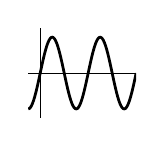
\begin{tikzpicture}[scale=0.2]
                    \begin{axis}[
                        axis lines*=middle,
                        ticks=none,
                        samples=100,
                        xmin=-0.5*pi, xmax=4*pi,
                        ymin=-1.25, ymax=1.25,
                        axis line style={line width=2pt}
                    ]
                    \addplot[
                        color=black,
                        domain=-0.5*pi:4*pi,
                        line width=5pt
                    ] {sin(deg(x))};
                    \end{axis}    
                \end{tikzpicture}
                \\
                \footnotesize{$y=sin(x)$}
            \end{minipage}\hfill

            \begin{minipage}[b]{0.2\linewidth}
                \centering
                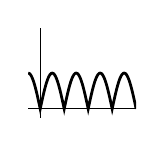
\begin{tikzpicture}[scale=0.2]
                    \begin{axis}[
                        axis lines*=middle,
                        ticks=none,
                        samples=100,
                        xmin=-0.5*pi, xmax=4*pi,
                        ymin=-0.25, ymax=2.25,
                        axis line style={line width=2pt}
                    ]
                    \addplot[
                        color=black,
                        domain=-0.5*pi:4*pi,
                        line width=5pt
                    ] {abs(sin(deg(x)))};
                    \end{axis}    
                \end{tikzpicture}
                \\
                \footnotesize{$y=\left\lvert x \right\rvert$}
            \end{minipage}\hfill

            \begin{minipage}[b]{0.2\linewidth}
                \centering
                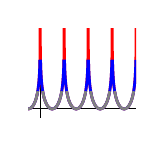
\begin{tikzpicture}[scale=0.2]
                    \begin{axis}[
                        axis lines*=middle,
                        ticks=none,
                        samples=1000,
                        xmin=-0.5*pi, xmax=4*pi,
                        ymin=-0.25, ymax=2.25,
                        axis line style={line width=2pt}
                    ]
                    \addplot[
                        color=red,
                        domain=-0.5*pi:4*pi,
                        line width=5pt
                    ] {-log10(abs(sin(deg(x))))};
                    \addplot[
                        color=blue,
                        domain=-0.5*pi:4*pi,
                        restrict y to domain=0:1.5,
                        line width=5pt
                    ] {-log10(abs(sin(deg(x))))};
                    \addplot[
                        color=black!50,
                        domain=-0.5*pi:4*pi,
                        restrict y to domain=0:0.5,
                        line width=5pt
                    ] {-log10(abs(sin(deg(x))))};
                    \end{axis}    
                \end{tikzpicture}
                \\
                \footnotesize{$y=-\log _{10}(x)$}
            \end{minipage}\hfill

            \begin{minipage}[b]{0.2\linewidth}
                \centering
                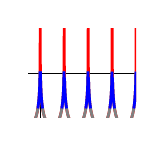
\begin{tikzpicture}[scale=0.2]
                    \begin{axis}[
                        axis lines*=middle,
                        ticks=none,
                        samples=1000,
                        xmin=-0.5*pi, xmax=4*pi,
                        ymin=-1.25, ymax=1.25,
                        axis line style={line width=2pt}
                    ]
                    \addplot[
                        color=red,
                        domain=-0.5*pi:4*pi,
                        line width=5pt
                    ] {-log10(abs(sin(deg(x))))-1.5};
                    \addplot[
                        color=black!50,
                        domain=-0.5*pi:4*pi,
                        restrict y to domain=-2:0.05,
                        line width=5pt
                    ] {-log10(abs(sin(deg(x))))-1.5};
                    \addplot[
                        color=blue,
                        domain=-0.5*pi:4*pi,
                        restrict y to domain=-1:0.05,
                        line width=5pt
                    ] {-log10(abs(sin(deg(x))))-1.5};
                    \end{axis}    
                \end{tikzpicture}
                \\
                \footnotesize{$y=x-T-\frac{W}{2}$}
            \end{minipage}\hfill

            \begin{minipage}[b]{0.2\linewidth}
                \centering
                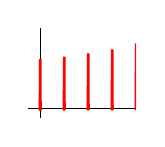
\begin{tikzpicture}[scale=0.2]
                    \begin{axis}[
                        axis lines*=middle,
                        ticks=none,
                        samples=5000,
                        xmin=-0.5*pi, xmax=4*pi,
                        ymin=-0.25, ymax=2.25,
                        axis line style={line width=2pt}
                    ]
                    \addplot[
                        color=red,
                        domain=-0.5*pi:4*pi,
                        line width=5pt,
                        restrict y to domain=-0.05:2.25,
                    ] {-log10(abs(sin(deg(x))))-1.5};
                    \end{axis}    
                \end{tikzpicture}
                \\
                \footnotesize{$y=\geq 0$}
            \end{minipage}\hfill

            \begin{minipage}[b]{0.2\linewidth}
                \centering
                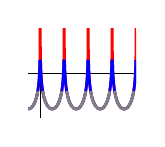
\begin{tikzpicture}[scale=0.2]
                    \begin{axis}[
                        axis lines*=middle,
                        ticks=none,
                        samples=1000,
                        xmin=-0.5*pi, xmax=4*pi,
                        ymin=-1.25, ymax=1.25,
                        axis line style={line width=2pt}
                    ]
                    \addplot[
                        color=red,
                        domain=-0.5*pi:4*pi,
                        line width=5pt
                    ] {-log10(abs(sin(deg(x))))-1};
                    \addplot[
                        color=blue,
                        domain=-0.5*pi:4*pi,
                        restrict y to domain=-1:0.5,
                        line width=5pt
                    ] {-log10(abs(sin(deg(x))))-1};
                    \addplot[
                        color=black!50,
                        domain=-0.5*pi:4*pi,
                        restrict y to domain=-1:-0.5,
                        line width=5pt
                    ] {-log10(abs(sin(deg(x))))-1};
                    \end{axis}    
                \end{tikzpicture}
                \\
                \footnotesize{$y=x-T$}
            \end{minipage}\hfill

            \begin{minipage}[b]{0.2\linewidth}
                \centering
                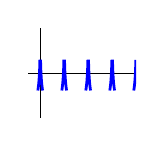
\begin{tikzpicture}[scale=0.2]
                    \begin{axis}[
                        axis lines*=middle,
                        ticks=none,
                        samples=1000,
                        xmin=-0.5*pi, xmax=4*pi,
                        ymin=-1.25, ymax=1.25,
                        axis line style={line width=2pt}
                    ]
                    \addplot[
                        color=blue,
                        domain=-0.5*pi:4*pi,
                        restrict y to domain=-0.5:0.5,
                        line width=5pt
                    ] {-log10(abs(sin(deg(x))))-1};
                    \end{axis}    
                \end{tikzpicture}
                \\
                \footnotesize{$-\frac{W}{2}\leq y \leq\frac{W}{2}$}
            \end{minipage}\hfill

            \begin{minipage}[b]{0.2\linewidth}
                \centering
                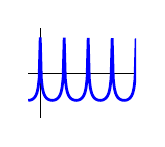
\begin{tikzpicture}[scale=0.2]
                    \begin{axis}[
                        axis lines*=middle,
                        ticks=none,
                        samples=100,
                        xmin=-0.5*pi, xmax=4*pi,
                        ymin=-1.25, ymax=1.25,
                        axis line style={line width=2pt}
                    ]
                    \addplot[
                        color=blue,
                        domain=-0.5*pi:4*pi,
                        line width=5pt
                    ] {tanh(-log10(abs(sin(deg(x))))-1)};
                    \end{axis}    
                \end{tikzpicture}
                \\
                \footnotesize{$y=tanh(x)$}
            \end{minipage}\hfill

            \caption{Transient signal throughout the attenuation calculator.}
            \label{fig:drc-diagram}

        \end{figure*}
        \fi

    \end{multicols*}

    \newpage

    \section*{Addendum}
        \textcolor{blue}{Put pictures of completed project, PCB layout, etc. over here.}

\end{document}